\documentclass{article}
\usepackage[utf8]{inputenc}
\usepackage{amsmath}
\usepackage{enumitem}
\usepackage{graphicx}
\usepackage{framed}
\usepackage{listings}
\usepackage{pdfpages}
\usepackage{caption}
\usepackage{subcaption}
\usepackage[utf8]{inputenc}
\usepackage{minted}
\usepackage{placeins}
\usepackage[utf8]{inputenc}


\title{Ch 9 Group Part 1}
\author{Tate Meehan, Arash Modaresi Rad, William Rudisill}
\date{March 2019}

\begin{document}

\maketitle

\section{The Equation}
We intend to solve the Van Genutchen equation, which is a nonlinear function that models the volumetric water content of a soil, $\theta$ (i.e, the fraction of a soil sample's total volume that is occupied by liquid water) as a function of water pressure (called pressure head) denoted by $h$. There are five parameters associated with the equation: $\alpha$, $\theta_s$, $\theta_r$, $n$, and $m$. 

The equation is given by:

\begin{align}
\theta = \theta_r + \frac{\theta_s - \theta_r}{\big(1 + |\alpha h|^n\big)^m}
\end{align}

\section{The Dataset}
We have data from the UNSODA soil database for $\theta$ and $h$ for a variety of different soils. 
\begin{figure}
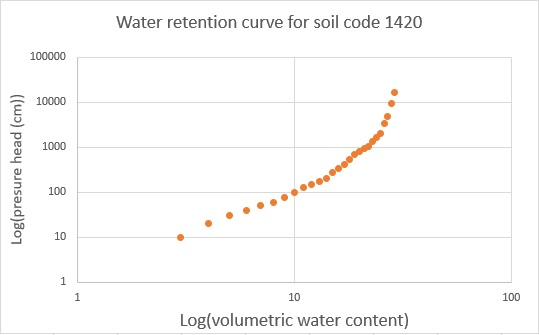
\includegraphics[]{soil.jpg}
\caption{$log(\theta)$ versus $log(h)$}
\end{figure}


\end{document}
